\chapter{\babLima}

\section{Analisis Pengujian Autentikasi  VxLang}
\subsection{Analisis Statis}
Analisis statis dilakukan untuk memahami mekanisme autentikasi aplikasi tanpa menjalankan kode. Alat yang digunakan dalam analisis ini adalah Ghidra, sebuah \f{software reverse engineering} yang menyediakan kemampuan \f{disassembly} dan \f{decompilation}. Tujuan utama dari analisis statis ini adalah untuk mengidentifikasi lokasi kode yang menangani proses autentikasi dan mencari potensi celah keamanan yang dapat dimanfaatkan untuk melewati proses tersebut.

\subsubsection{Analisis Aplikasi Non-Virtualized}
Pada aplikasi non-virtualized (konsol, Qt, dan ImGUI), proses analisis dimulai dengan mencari \f{string} yang relevan dengan autentikasi, seperti "Authentication Failed" atau \f{string} yang mungkin digunakan sebagai \f{username} atau \f{password}. Setelah \f{string} tersebut ditemukan, langkah selanjutnya adalah menelusuri referensi silang (\f{cross-references}) untuk melihat di mana \f{string} tersebut digunakan dalam kode program. Hal ini membantu dalam mengidentifikasi fungsi atau blok kode yang bertanggung jawab untuk menampilkan pesan kegagalan autentikasi, yang sering kali berdekatan dengan logika autentikasi itu sendiri.

Sebagai contoh, pada aplikasi \textit{app\_imgui}, analisis \f{disassembly} menggunakan Ghidra mengungkapkan potongan kode berikut:

\begin{listing}[H]
    \begin{minted}{asm}
; (Kode memuat input password ke register, misal RDI) ...

; (Kode memuat password hardcoded "rahman", misal ke alamat yg ditunjuk RDX)

LEA            RDX,[s_rahman_140110551]   = "rahman"
MOV            RCX,RDI
CALL           VCRUNTIME140.DLL::memcmp ; Bandingkan input & hardcoded pwd
CMP            RBX,0x6
TEST           EAX,EAX                  ; Cek hasil memcmp (EAX=0 jika sama)
JNZ            LAB_140003226            ; Lompat ke blok gagal jika EAX != 0

; (Blok kode jika autentikasi berhasil) 

LAB_140003226:  ; Label untuk blok gagal
LEA            RDX,[u_Authentication_Failed_1401104da] ; Load string "Auth Failed"
CALL           qword ptr [->USER32.DLL::MessageBoxW] ; Tampilkan pesan gagal

\end{minted}
\caption{Snippet Assembly: Perbandingan Password dan Lompatan Kondisional (Non-Virtualized)}
\label{lst:asm_static_nonvirt_snippet_updated} % Pastikan label unik jika ada versi lama
\end{listing}

Dalam konteks kode di atas, pemanggilan \code{memcmp} (di operasi \texttt{LEA}) membandingkan password yang dimasukkan pengguna dengan nilai "rahman" yang \textit{hardcoded} pada aplikasinya. Hasilnya diperiksa oleh \code{TEST EAX,EAX} (\texttt{140003216}). Jika password tidak sama, \code{EAX} tidak akan nol, dan instruksi \code{JNZ} (\texttt{140003218}, Jump if Not Zero) akan mengalihkan eksekusi ke \code{LAB\_140003226}, di mana pesan "Authentication Failed" ditampilkan. 

Untuk memvalidasi potensi celah keamanan, instruksi `JNZ LAB\_140003226` dapat diubah (\f{patched}) menjadi `JZ LAB\_140003226` atau instruksi lain yang akan selalu mengarahkan program untuk melewati blok kode yang menampilkan pesan kegagalan autentikasi. Dalam kasus ini, mengubah `JNZ` menjadi `JZ` (Jump if Zero) akan menyebabkan lompatan terjadi hanya jika hasil perbandingan adalah nol (yang menandakan autentikasi berhasil), sehingga secara efektif membalikkan logika dan memungkinkan akses tanpa otorisasi.

Lebih lanjut, analisis pada bagian \f{defined data} (.rdata) juga mengungkapkan adanya \f{string} `"seno"` dan `"rahman"`. Keberadaan \f{string-string} ini sangat mengindikasikan bahwa aplikasi menyimpan \f{username} dan \f{password} secara \f{hard-coded}. Praktik menyimpan kredensial secara langsung dalam kode program sangat berbahaya dari sudut pandang keamanan. String seperti ini mudah ditemukan melalui analisis statis, seperti yang telah dilakukan, sehingga penyerang dapat dengan mudah memperoleh informasi \f{username} dan \f{password} tanpa perlu melakukan \f{reverse engineering} yang mendalam atau menjalankan aplikasi. Dalam kasus ini, \f{username} `"seno"` dan \f{password} `"rahman"` yang ditemukan dalam \f{defined data} dapat dieksploitasi untuk melewati mekanisme autentikasi.

\begin{figure}[H] % Ganti H dengan htbp jika ingin float
	\centering
	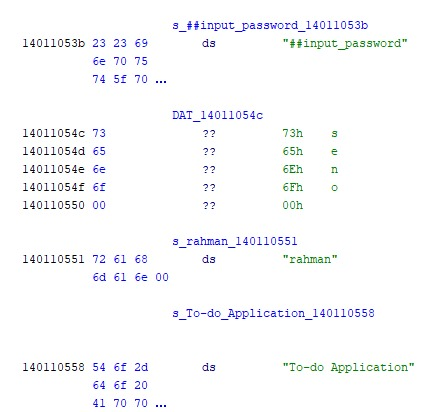
\includegraphics[width=0.45\textheight]
	{\Assets/hardcoded_credentials.jpeg}
  \caption{\f{Hardcoded username \& password} pada \f{defined data}}
\end{figure}

Analisis serupa juga dilakukan pada aplikasi konsol dan Qt, di mana pola perbandingan string dan penggunaan instruksi kondisional untuk mengontrol alur program berdasarkan hasil autentikasi juga ditemukan dan dapat dimanipulasi dengan cara yang serupa untuk melewati proses autentikasi.

\subsubsection{Analisis Aplikasi Non-Virtualized (Versi Cloud)}
Untuk mengatasi risiko \f{hard-coded} username dan password, mekanisme autentikasi telah diubah menjadi berbasis \f{cloud}. Dalam versi \f{cloud} ini, aplikasi mengirimkan username dan password dalam format JSON ke server HTTP, yang kemudian melakukan verifikasi terhadap database PostgreSQL. Dengan perubahan ini, username dan password tidak lagi disimpan secara langsung di dalam aplikasi klien.

Meskipun kredensial tidak lagi \f{hard-coded}, analisis statis tetap relevan untuk memahami bagaimana aplikasi klien berinteraksi dengan server. Sebagai contoh, pada aplikasi \textit{console\_cloud}, analisis \f{disassembly} menggunakan Ghidra pada fungsi yang menangani autentikasi menunjukkan potongan kode berikut:

\begin{listing}[H]
    \begin{minted}[linenos=false]{asm}
; ... (Kode setelah fungsi send_login_request kembali, hasil mungkin di AL) ...
MOV      AL, byte ptr [RBP + local_69] ; Ambil hasil boolean?
TEST     AL, 0x1                       ; Cek bit 0 dari AL
JNZ      LAB_14000175d                 ; Lompat jika hasil != 0 (Sukses?)
JMP      LAB_14000178e                 ; Lompat jika hasil == 0 (Gagal?)

LAB_14000175d:  ; Blok kode jika sukses
; ... (Kode menampilkan "Authorized!") ...
jmp      LAB_END_AUTH_CHECK                       ; Lompat ke akhir

LAB_14000178e:  ; Blok kode jika gagal
; ... (Kode menampilkan "Not authorized") ...

\end{minted}
\caption{Snippet Assembly: Pemeriksaan Hasil Autentikasi Cloud (Non-Virtualized)}
\label{lst:asm_static_cloud_snippet_updated} % Pastikan label unik
\end{listing}

Pada kode di atas, instruksi \code{TEST AL, 0x1} kemungkinan memeriksa flag atau nilai boolean yang dikembalikan oleh fungsi autentikasi cloud (misalnya, 1 untuk sukses, 0 untuk gagal). Instruksi \code{JNZ LAB\_14000175d} kemudian mengarahkan alur eksekusi ke blok "Authorized!" jika hasil tes tidak nol (sukses), dan sebaliknya akan jatuh ke \code{JMP LAB\_14000178e} atau langsung mengeksekusi blok "Not authorized". Sama seperti kasus sebelumnya, instruksi \code{JNZ} ini dapat dimanipulasi (misal, diubah menjadi \code{JMP LAB\_14000175d} atau \code{NOP}) untuk memaksa alur ke blok sukses, meskipun server menolak autentikasi. Konteks assembly yang lebih lengkap dapat dilihat pada Lampiran \ref{app:kode_asm} (Kode \ref{lst:asm_static_cloud_full}).

Sama seperti pada kasus \f{hard-coded} sebelumnya, instruksi `JNZ LAB\_14000175d` dapat diubah menjadi `JZ LAB\_14000175d`. Dengan perubahan ini, program akan selalu melompat ke bagian yang menampilkan "Authorized!" tanpa perlu melakukan verifikasi yang sebenarnya dari server. Meskipun username dan password tidak lagi disimpan di dalam aplikasi, logika di sisi klien yang menentukan apakah autentikasi berhasil atau gagal masih dapat dimanipulasi.

Ini menunjukkan bahwa meskipun memindahkan logika autentikasi ke server dan menghindari \f{hard-coded credential} meningkatkan keamanan, sisi klien aplikasi masih dapat menjadi target untuk \f{reverse engineering}. Penyerang dapat memodifikasi aplikasi klien untuk selalu menganggap autentikasi berhasil, meskipun server mungkin menolak permintaan autentikasi. Oleh karena itu, keamanan menyeluruh memerlukan perlindungan tidak hanya pada kredensial tetapi juga pada logika bisnis aplikasi di sisi klien.

Analisis serupa juga dilakukan pada aplikasi konsol dan ImGUI versi \f{cloud}, di mana pola pemeriksaan kondisi dan jump kondisional yang menentukan status autentikasi juga ditemukan dan berpotensi untuk dimanipulasi.

\subsubsection{Analisis Aplikasi Virtualized}

Analisis statis pada aplikasi yang telah divirtualisasi menggunakan VxLang menunjukkan tingkat kesulitan yang jauh lebih tinggi dibandingkan versi non-virtualized. Observasi kualitatif sebelumnya diperkuat oleh data kuantitatif yang diperoleh dari ringkasan analisis Ghidra terhadap \f{executable} \code{app\_qt.exe} (asli) dan \code{app\_qt\_vm.exe} (virtualized), seperti yang dirangkum dalam Gambar \ref{fig:ghidra_summary_qt_bab5} dan \ref{fig:ghidra_summary_qt_vm_bab5}.

Beberapa temuan kuantitatif dan kualitatif signifikan adalah:

\begin{itemize}
    \item \bo{Hilangnya Informasi Struktural Fundamental:} Perbedaan paling mencolok adalah Ghidra melaporkan \textbf{0 instruksi} dan \textbf{0 fungsi} yang terdeteksi pada \code{app\_qt\_vm.exe}, dibandingkan dengan 9133 instruksi dan 678 fungsi pada \code{app\_qt.exe} (lihat Gambar \ref{fig:ghidra_summary_qt_bab5} dan \ref{fig:ghidra_summary_qt_vm_bab5}). Hal ini secara fundamental mengindikasikan bahwa Ghidra tidak dapat menginterpretasikan atau me-\f{disassemble} \f{bytecode} yang dihasilkan oleh VxLang sebagai instruksi mesin x86-64 standar. Akibatnya, pemahaman alur kontrol program dan identifikasi blok logika menjadi hampir mustahil melalui analisis statis konvensional.

    \item \bo{Penurunan Drastis Data Terdefinisi dan Simbol:} Jumlah data yang terdefinisi (\f{Defined Data}) berkurang signifikan dari 1987 pada versi asli menjadi hanya 128 pada versi virtualized. Demikian pula, jumlah simbol yang dikenali turun drastis dari 2761 menjadi 23. Penurunan ini secara kuantitatif mendukung observasi sebelumnya mengenai hilangnya \f{string-string} penting (seperti "Authentication Failed") dan nama-nama fungsi atau variabel yang dapat membantu analisis. Ini menunjukkan bahwa VxLang efektif menyembunyikan atau mengenkripsi data dan mengaburkan titik masuk serta referensi internal program.

    \item \bo{Peningkatan Ukuran File yang Substansial:} Ukuran \f{executable} \code{app\_qt} meningkat secara masif dari sekitar 122 KB  menjadi sekitar 1.578 KB. Peningkatan ukuran sekitar 12.9 kali lipat ini kemungkinan besar disebabkan oleh penyertaan \f{runtime} atau \f{interpreter} mesin virtual VxLang beserta representasi \f{bytecode} dari kode asli yang divirtualisasi.

    \item \bo{Kesulitan Identifikasi Struktur Kode Lainnya:} Penurunan jumlah tipe data (dari 428 menjadi 37) dan kategori tipe data (dari 28 menjadi 3) juga menunjukkan hilangnya informasi struktural yang biasanya dapat diekstraksi oleh Ghidra. Selain itu, Ghidra tidak dapat lagi mengidentifikasi \f{compiler} asli (clang), menandakan perubahan signifikan pada struktur \f{header} dan metadata \f{executable}.

    \item \bo{Operasi yang Tidak Diketahui Tetap Ada:} Meskipun ringkasan menunjukkan 0 instruksi, saat menjelajahi kode secara manual di Ghidra, banyak operasi \f{assembly} yang tidak dikenali atau dikategorikan sebagai '???' tetap muncul, seperti yang diobservasi sebelumnya. Ini semakin memperkuat gagasan bahwa kode telah ditransformasi menjadi format yang tidak standar.
\end{itemize}

% --- GAMBAR GHIDRA SUMMARY QT ASLI (BAB 5) ---
\begin{figure}[H] % Ganti H dengan htbp jika ingin float
    \centering
    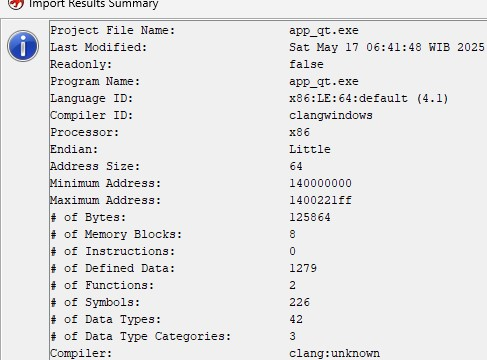
\includegraphics[width=0.9\textwidth]{\Assets/app_qt_summary_result.jpeg} % Sesuaikan path dan ukuran
    \caption{Ringkasan Hasil Analisis Ghidra untuk \code{app\_qt.exe} (Non-Virtualized).}
    \label{fig:ghidra_summary_qt_bab5}
\end{figure}
% --- AKHIR GAMBAR GHIDRA SUMMARY QT ASLI (BAB 5) ---

% --- GAMBAR GHIDRA SUMMARY QT VM (BAB 5) ---
\begin{figure}[H] % Ganti H dengan htbp jika ingin float
    \centering
    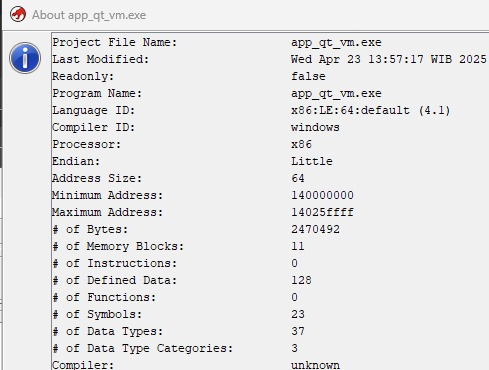
\includegraphics[width=0.9\textwidth]{\Assets/app_qt_vm_summary_result.jpeg} % Sesuaikan path dan ukuran
    \caption{Ringkasan Hasil Analisis Ghidra untuk \code{app\_qt\_vm.exe} (Virtualized).}
    \label{fig:ghidra_summary_qt_vm_bab5}
\end{figure}
% --- AKHIR GAMBAR GHIDRA SUMMARY QT VM (BAB 5) ---

Secara keseluruhan, data kuantitatif dari Ghidra ini memberikan bukti kuat bahwa \f{code virtualization} menggunakan VxLang secara efektif mengaburkan struktur fundamental program pada tingkat biner. Ketidakmampuan \f{disassembler/decompiler} seperti Ghidra untuk mengenali instruksi, fungsi, dan data secara signifikan meningkatkan kesulitan analisis statis. Identifikasi dan manipulasi logika autentikasi melalui pendekatan statis konvensional menjadi sangat tidak praktis dan kemungkinan besar tidak berhasil pada aplikasi yang telah divirtualisasi dengan VxLang.

\subsection{Analisis Dinamis}
Analisis dinamis dilakukan dengan menjalankan aplikasi di bawah \f{debugger} x64dbg untuk mengamati perilaku saat \f{runtime}. Tujuannya adalah untuk memverifikasi temuan dari analisis statis dan memahami bagaimana aplikasi berinteraksi dengan \f{input} pengguna, khususnya dalam proses autentikasi.

\subsubsection{Analisis Aplikasi Non-Virtualized}

Untuk aplikasi non-virtualized, analisis dinamis dilakukan dengan mencari string yang relevan dengan proses autentikasi, seperti username dan password yang ditemukan pada analisis statis ("seno" dan "rahman"). \f{Breakpoint} dipasang pada lokasi di mana \f{string} ini digunakan atau dibandingkan.

Pada aplikasi \textit{app\_qt}, saat dijalankan di bawah x64dbg dan diberikan \f{input} yang salah, \f{debugger} mengarahkan eksekusi ke blok kode berikut:

\begin{listing}[H]
    \begin{minted}[linenos=false]{asm}
; ... (Kode membandingkan input password dengan "rahman" via operator==) ...
; Hasil perbandingan (boolean) mungkin disimpan di AL atau flag register

mov al, byte ptr ss:[rbp-41]  ; Ambil hasil perbandingan
test al, 1                    ; Cek apakah hasilnya true (misal: 1)

; Perhatikan bahwa logika JNE/JE mungkin berbeda tergantung optimasi compiler
; Asumsi: JNE melompat jika perbandingan GAGAL (tidak sama)

jne SHORT failure_label       ; Lompat ke blok GAGAL jika password TIDAK sama
; ... (Kode jika password BENAR) ...

jmp END_OF_AUTH

failure_label:
; ... (Kode setup untuk menampilkan "Authentication Failed" via QMessageBox) ...

lea rdx, qword ptr ds:[<"Authentication Failed">]
; ... (call ke fungsi QMessageBox) ...

\end{minted}
\caption{Snippet Assembly: Lompatan Kondisional Setelah Perbandingan Password (Dinamis, Non-Virtualized)}
\label{lst:asm_dynamic_nonvirt_snippet_updated} % Pastikan label unik
\end{listing}

Instruksi \code{test al, 1} memeriksa hasil perbandingan password. Jika password salah (misalnya, \code{al} adalah 0), instruksi \code{jne failure\_label} (Jump if Not Equal/Zero) akan dieksekusi, mengarahkan program ke blok yang menampilkan "Authentication Failed". Dalam analisis dinamis, \textit{debugger} seperti x64dbg memungkinkan \textit{patching on-the-fly}. Dengan mengubah instruksi \code{jne} menjadi \code{je} (Jump if Equal/Zero) atau \code{jmp} (lompatan tanpa syarat ke blok sukses), pemeriksaan password dapat dilewati secara efektif saat \textit{runtime}. Konteks assembly yang lebih lengkap dari sesi debugging ini dapat dilihat di Lampiran \ref{app:kode_asm} (Kode \ref{lst:asm_dynamic_nonvirt_full}).

Sama seperti pada analisis statis, celah keamanan dapat dieksploitasi dengan memodifikasi alur eksekusi. Dalam x64dbg, instruksi `jne` dapat diubah menjadi `je` (Jump if Equal) secara langsung pada saat \f{runtime}. Dengan melakukan perubahan ini, program akan melompat ke bagian yang seharusnya dijalankan hanya jika autentikasi berhasil, meskipun \f{input} yang diberikan salah. Operasi negasi ini secara efektif melewati pemeriksaan autentikasi.

\subsubsection{Analisis Aplikasi Virtualized}

Analisis dinamis pada aplikasi yang telah divirtualisasi menggunakan x64dbg menunjukkan tantangan yang serupa dengan analisis statis. Ketika mencari string seperti "Authentication Failed", \f{debugger} sering kali tidak dapat menemukannya dalam memori proses. Hal ini mengindikasikan bahwa string tersebut mungkin tidak disimpan dalam format yang jelas atau mungkin dienkripsi dan didekripsi hanya pada saat digunakan.

Selain itu, x64dbg juga menampilkan banyak operasi dengan kategori ??? yang tidak dapat di-\f{disassemble}. Hal ini mempersulit pemahaman alur eksekusi dan fungsi-fungsi yang terlibat dalam proses autentikasi.

Lebih lanjut, melacak alur eksekusi saat memasukkan username dan password menjadi sangat sulit. Berikut adalah perbandingan \f{section} kode saat menerima \f{input} pada aplikasi konsol non-virtualized dan virtualized:


\bo{Non-Virtualized:} Menampilkan panggilan standar ke fungsi I/O C++.
\begin{listing}[H]
    \begin{minted}[linenos=false]{asm}
; ...
mov rcx,qword ptr ds:[<...std::cout>]      ; Pointer ke std::cout
lea rdx,qword ptr ds:[<"Enter username: ">] ; Pointer ke string prompt
call <console. ... std::operator<< ...>    ; Panggil fungsi print (std::cout << prompt)
; ...
mov rcx,qword ptr ds:[<...std::cin>]       ; Pointer ke std::cin
lea rdx,qword ptr ss:[rbp-28]              ; Pointer ke buffer input string
call <console. ... std::operator>> ...>    ; Panggil fungsi read (std::cin >> buffer)
; ...
\end{minted}
\caption{Snippet Assembly: Operasi Input/Output Standar (Non-Virtualized)}
\label{lst:asm_dynamic_io_nonvirt_snippet_updated} % Pastikan label unik
\end{listing}

\bo{Virtualized:} Menampilkan instruksi yang diobfuskasi dan sulit dikenali oleh debugger.
\begin{listing}[H]
    \begin{minted}[linenos=false]{asm}
??? ; Operasi tidak dikenal
jmp console_vm.vxm.7FF74CD97168 ; Lompatan internal VM?
fcmovnu st(0),st(5) ; Operasi FPU tidak relevan?
xor byte ptr ds:[rsi],ah ; Operasi XOR
??? ; Operasi tidak dikenal
jmp console_vm.vxm.7FF74CD48254 ; Lompatan pendek
fstp st(0) ; Operasi FPU
\end{minted}
\caption{Snippet Assembly: Instruksi di Lokasi Input (Virtualized)}
\label{lst:asm_dynamic_io_virt_snippet_updated} % Pastikan label unik
\end{listing}

Perbandingan ini menunjukkan kontras yang jelas. Pada kode non-virtualized, panggilan ke fungsi I/O standar seperti \code{std::cout} dan \code{std::cin} mudah dikenali. Sebaliknya, pada kode yang telah divirtualisasi, instruksi assembly menjadi tidak jelas (\code{???}), diselingi dengan lompatan (\code{jmp}) dan operasi lain yang tampaknya tidak berhubungan langsung dengan I/O (\code{fcmovnu}, \code{xor}, \code{fstp}). Hal ini menyulitkan pelacakan alur eksekusi saat input dimasukkan. Lebih lanjut, observasi menunjukkan register RIP (\f{Instruction Pointer}) seringkali tampak "\f{stuck}" pada alamat tertentu dalam \textit{debugger}, mengindikasikan eksekusi kemungkinan terjadi di dalam \textit{interpreter} mesin virtual VxLang. Hal ini sangat menyulitkan untuk melacak alur eksekusi dan memahami apa yang sebenarnya terjadi di balik layar. Perilaku ini mengindikasikan bahwa VxLang menggunakan teknik virtualisasi yang kompleks, yang secara signifikan menghambat analisis dinamis menggunakan metode tradisional seperti mencari string dan memantau alur eksekusi secara langsung. Konteks assembly yang lebih lengkap untuk perbandingan ini dapat dilihat di Lampiran \ref{app:kode_asm} (Kode \ref{lst:asm_dynamic_io_comparison_full}).

\section{Analisis Performa \f{Overhead} VxLang}
Hasil dari percobaan performa overhead dan perubahan ukuran file setelah penerapan virtualisasi kode menggunakan VxLang. Percobaan ini dilakukan pada algoritma Quick Sort dan enkripsi AES-CBC-256.

\subsection{Hasil Pengujian Performa \f{Quick Sort}}
Tabel \ref{tab:quick_sort_performance_updated} menyajikan hasil pengukuran waktu rata-rata dan standar deviasi dari algoritma Quick Sort yang dijalankan sebanyak 100 kali untuk setiap ukuran array, baik sebelum maupun sesudah virtualisasi menggunakan VxLang. Data virtualisasi untuk ukuran array di atas 1.000.000 elemen tidak tersedia dalam log pengujian \textit{release build} ini.

\begin{table}[H] % Ganti H dengan htbp jika ingin float
    \centering
    \caption{Hasil Pengujian Waktu Eksekusi Quick Sort (ms)}
    \label{tab:quick_sort_performance_updated}
    \begin{tabularx}{\textwidth}{@{}|X|X|X|X|X|@{}}
    \hline
        \multirow{2}{*}{\textbf{Ukuran Array}} & \multicolumn{2}{c|}{\textbf{Tanpa Virtualisasi}} & \multicolumn{2}{c|}{\textbf{Dengan Virtualisasi}}\\
        \cline{2-5}
        & \textbf{Rata-rata Waktu (ms)} & \textbf{Standar Deviasi (ms)} & \textbf{Rata-rata Waktu (ms)} & \textbf{Standar Deviasi (ms)}\\
        \hline
        100                     & 0.01 & 0.00 & 2.74 & 0.38 \\
        \hline
        1,000                   & 0.08 & 0.00 & 27.35 & 1.25 \\
        \hline
        5,000                   & 0.54 & 0.05 & 144.44 & 8.25 \\
        \hline
        10,000                  & 1.24 & 0.08 & 295.77 & 13.68 \\
        \hline
        50,000                  & 6.98 & 0.51 & 1,556.15 & 122.81 \\
        \hline
        100,000                 & 15.12 & 1.26 & 3,080.30 & 303.02 \\
        \hline
        500,000                 & 104.44 & 7.30 & 14,298.92 & 374.98 \\
        \hline
        1,000,000               & 218.32 & 8.10 & 33,292.91 & 4,342.93 \\
        \hline
    \end{tabularx}
\end{table}

\begin{figure}[H] % Ganti H dengan htbp jika ingin float
    \centering
    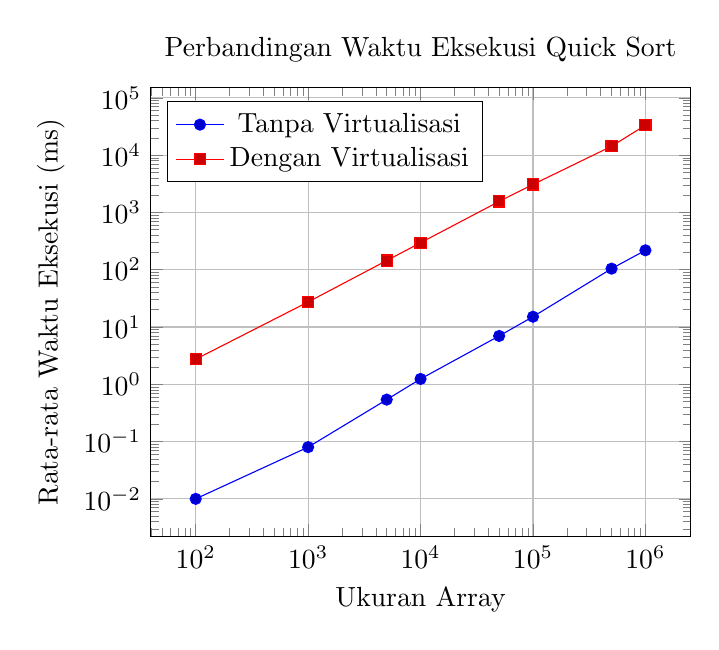
\begin{tikzpicture}
        \begin{axis}[
            xlabel={Ukuran Array},
            ylabel={Rata-rata Waktu Eksekusi (ms)},
            xmode=log,
            log basis x={10},
            ymode=log,
            log basis y={10},
            legend pos=north west,
            title={Perbandingan Waktu Eksekusi Quick Sort},
            grid=major,
        ]
        \addplot coordinates {
            (100, 0.01)
            (1000, 0.08)
            (5000, 0.54)
            (10000, 1.24)
            (50000, 6.98)
            (100000, 15.12)
            (500000, 104.44)
            (1000000, 218.32)
        };
        \addlegendentry{Tanpa Virtualisasi};

        \addplot coordinates {
            (100, 2.74)
            (1000, 27.35)
            (5000, 144.44)
            (10000, 295.77)
            (50000, 1556.15)
            (100000, 3080.30)
            (500000, 14298.92)
            (1000000, 33292.91)
        };
        \addlegendentry{Dengan Virtualisasi};
        \end{axis}
    \end{tikzpicture}
    \caption{Perbandingan Waktu Eksekusi Algoritma Quick Sort antara Versi Tanpa dan Dengan Virtualisasi VxLang.}
    \label{fig:quick_sort_performance_updated}
\end{figure}

Berdasarkan Tabel \ref{tab:quick_sort_performance_updated} dan Gambar \ref{fig:quick_sort_performance_updated}, terlihat adanya peningkatan waktu eksekusi yang sangat signifikan pada algoritma Quick Sort setelah divirtualisasi menggunakan VxLang, bahkan pada \textit{release build}. Peningkatan ini konsisten terjadi seiring dengan bertambahnya ukuran array. Sebagai contoh:
\begin{itemize}
    \item Untuk array berukuran 100 elemen, waktu eksekusi rata-rata meningkat dari 0.01 ms menjadi 2.74 ms, yang menunjukkan \textit{overhead} sekitar 27,300\%.
    \item Untuk array berukuran 100.000 elemen, waktu eksekusi meningkat dari 15.12 ms menjadi 3.080.30 ms, dengan \textit{overhead} sekitar 20,272\%.
    \item Untuk array terbesar yang diuji pada versi virtualisasi (1.000.000 elemen), waktu eksekusi meningkat dari 218.32 ms menjadi 33.292.91 ms, menghasilkan \textit{overhead} sekitar 15,150\%.
\end{itemize}
Peningkatan standar deviasi juga menunjukkan bahwa waktu eksekusi pada versi virtualisasi menjadi lebih bervariasi, terutama pada ukuran array yang lebih besar. Hal ini mengindikasikan adanya \textit{overhead} yang substansial dan kurang prediktabilitas yang diperkenalkan oleh mesin virtual VxLang dalam mengeksekusi instruksi virtual dibandingkan dengan eksekusi kode \textit{native}. Meskipun \textit{overhead} ini mungkin sedikit lebih rendah dibandingkan dengan \textit{debug build} sebelumnya (misalnya, untuk 1 juta elemen, \textit{overhead debug build} adalah sekitar 20.860\%), nilainya tetap sangat tinggi dan menunjukkan dampak performa yang berat.

\subsection{Hasil Pengujian Performa Enkripsi AES-CBC-256}
Tabel \ref{tab:aes_performance_updated} menyajikan hasil benchmarking enkripsi AES-CBC-256 dengan 1.000.000 blok data (total 976 MB), sebelum dan sesudah virtualisasi menggunakan VxLang.

\begin{table}[H] % Ganti H dengan htbp jika ingin float
  \centering
  \caption{Hasil Pengujian Performa Enkripsi AES-CBC-256}
  \label{tab:aes_performance_updated}
  \begin{tabular}{|l|c|c|}
    \hline
    \bo{Metrik}                                     & \bo{Tanpa Virtualisasi} & \bo{Dengan Virtualisasi} \\
    \hline
    Total Waktu Enkripsi (ms)                  & 1,878.52            & 9,330.73            \\
    \hline
    Total Waktu Dekripsi (ms)                  & 1,304.75            & 8,649.74            \\
    \hline
    Rata-rata Waktu per Blok Enkripsi (ms)     & 0.00188            & 0.00933             \\ % Dihitung dari total waktu / 1jt blok
    \hline
    Rata-rata Waktu per Blok Dekripsi (ms)     & 0.00130            & 0.00865             \\ % Dihitung dari total waktu / 1jt blok
    \hline
    \textit{Throughput} Enkripsi (MB/s)               & 519.86             & 104.66               \\
    \hline
    \textit{Throughput} Dekripsi (MB/s)               & 748.46             & 112.90               \\
    \hline
    \textit{Throughput} Gabungan (MB/s)               & 634.16             & 108.78               \\
    \hline
  \end{tabular}
\end{table}

Hasil pengujian enkripsi AES-CBC-256 pada \textit{release build} juga menunjukkan \textit{overhead} performa yang signifikan setelah penerapan VxLang.
\begin{itemize}
    \item Total waktu enkripsi meningkat dari 1.878.52 ms menjadi 9.330.73 ms, yang merupakan peningkatan sekitar 396.7\%.
    \item Total waktu dekripsi mengalami peningkatan dari 1.304.75 ms menjadi 8.649.74 ms, atau sekitar 562.9\%.
\end{itemize}
Peningkatan waktu eksekusi ini berdampak langsung pada penurunan \textit{throughput} (kecepatan pemrosesan data):
\begin{itemize}
    \item \textit{Throughput} enkripsi menurun dari 519.86 MB/s menjadi 104.66 MB/s (penurunan sekitar 79.9\%).
    \item \textit{Throughput} dekripsi menurun dari 748.46 MB/s menjadi 112.90 MB/s (penurunan sekitar 84.9\%).
    \item \textit{Throughput} gabungan (rata-rata enkripsi dan dekripsi) menurun dari 634.16 MB/s menjadi 108.78 MB/s, yang merupakan penurunan sekitar 82.8\%.
\end{itemize}
Hasil ini mengkonfirmasi bahwa virtualisasi kode dengan VxLang memperkenalkan \textit{overhead} yang cukup besar pada operasi komputasi intensif seperti enkripsi, bahkan dalam \textit{release build} yang umumnya lebih teroptimasi dibandingkan \textit{debug build}. Perbandingkan dengan \textit{debug build} sebelumnya (enkripsi +384\%, dekripsi +510\%, throughput gabungan turun 82%), angka-angka pada \textit{release build} ini menunjukkan pola \textit{overhead} yang serupa dan tetap signifikan.

\subsection{Hasil Pengujian Ukuran File}
Tabel \ref{tab:file_size_updated} menyajikan ukuran file \f{executable} (dalam KB) untuk berbagai program sebelum dan sesudah virtualisasi menggunakan VxLang.

\begin{table}[htbp]
  \centering
  \caption{Hasil Pengujian Ukuran File (KB)}
  \label{tab:file_size_updated}
  \begin{tabular}{@{}|l|c|c|@{}}
    \hline
    \multirow{2}{*}{\textbf{Program}} & \multicolumn{2}{c|}{\textbf{Ukuran File}} \\
    \cline{2-3} & \bo{Tanpa Virtualisasi} & \bo{Virtualiasi} \\
    \hline
    quick\_sort        & 98       & 1,537     \\
    \hline
    encryption         & 110      & 1,507     \\
    \hline
    size               & 97,771   & 112,324   \\
    \hline
    console            & 92       & 1,577     \\
    \hline
    console\_cloud      & 281      & 1,695     \\
    \hline
    app\_imgui         & 1,675    & 2,330     \\
    \hline
    app\_imgui\_cloud    & 1,860    & 2,418     \\
    \hline
    app\_qt            & 122      & 1,578     \\
    \hline
    app\_qt\_cloud       & 315      & 1,671     \\
    \hline
    Lilith\_Client     & 84       & 1,554     \\
    \hline
  \end{tabular}
\end{table}

Hasil pengukuran ukuran file pada \textit{release build} menunjukkan bahwa penerapan virtualisasi kode menggunakan VxLang secara konsisten meningkatkan ukuran file \textit{executable}.
\begin{itemize}
    \item Untuk program-program kecil dan sederhana seperti \texttt{quick\_sort} (98 KB menjadi 1.537 KB, peningkatan sekitar 15.7x), \texttt{console} (92 KB menjadi 1.577 KB, peningkatan sekitar 17.1x), dan \texttt{Lilith\_Client} (84 KB menjadi 1.554 KB, peningkatan sekitar 18.5x), peningkatannya sangat signifikan, seringkali lebih dari 15 kali lipat.
    \item Untuk aplikasi GUI yang lebih besar atau yang menggunakan library eksternal seperti \texttt{app\_imgui} (1.675 KB menjadi 2.330 KB, peningkatan sekitar 1.39x) dan \texttt{app\_qt\_cloud} (315 KB menjadi 1.671 KB, peningkatan sekitar 5.3x), persentase peningkatannya lebih kecil, namun absolutnya tetap menunjukkan penambahan ukuran yang cukup besar (ratusan hingga ribuan KB).
    \item Aplikasi \texttt{size} yang dirancang dengan aset data tersemat besar (97.771 KB) menunjukkan peningkatan ukuran yang relatif paling kecil secara persentase (menjadi 112.324 KB, peningkatan sekitar 1.15x atau 15\%), namun ini tetap berarti penambahan sekitar 14.5 MB. Ini mengindikasikan bahwa \textit{overhead} utama berasal dari \textit{runtime} VxLang itu sendiri, dan dampaknya lebih terasa pada aplikasi kecil.
\end{itemize}
Peningkatan ukuran ini, seperti pada \textit{debug build}, kemungkinan besar disebabkan oleh penambahan \textit{interpreter} mesin virtual VxLang dan representasi \textit{bytecode} dari kode asli ke dalam \textit{executable} yang dilindungi. Peningkatan ini konsisten di semua jenis aplikasi yang diuji.

\section{Analisis Aplikasi RAT Lilith dengan VxLang}
\label{bab:hasil_penelitian_lilith_updated} % Pastikan label unik jika perlu
Bagian ini menyajikan hasil analisis terhadap aplikasi RAT Lilith, baik dalam versi asli maupun versi yang telah divirtualisasi menggunakan VxLang. Analisis mencakup evaluasi kesulitan \textit{reverse engineering} secara statis dan dinamis, serta dampak virtualisasi terhadap deteksi oleh layanan pemindaian \textit{malware} VirusTotal.

\subsection{Analisis Statis dan Dinamis RAT Lilith}
\label{subsec:analisis_statdin_lilith_updated} % Pastikan label unik jika perlu
Analisis statis menggunakan Ghidra dan analisis dinamis menggunakan x64dbg dilakukan pada kedua versi klien Lilith.
\begin{itemize}
    \item \textbf{RAT Lilith Non-Virtualized:} Analisis terhadap versi asli Lilith relatif mudah dilakukan. \textit{String} terkait fungsionalitasnya (misalnya, perintah-perintah, pesan status) dapat ditemukan. Alur kontrol untuk pemrosesan perintah dan komunikasi jaringan dapat dilacak. Dengan pemahaman yang cukup, seorang analis dapat mengidentifikasi mekanisme \textit{keylogging}, cara kerja perintah \textit{remote control}, dan bagaimana data dikirimkan antara klien dan server.
    \item \textbf{RAT Lilith Virtualized:} Sejalan dengan temuan pada aplikasi studi kasus autentikasi, versi Lilith yang telah divirtualisasi menunjukkan peningkatan kesulitan analisis yang signifikan:
        \begin{itemize}
            \item \textbf{Analisis Statis (Ghidra):} Sebagian besar instruksi dalam fungsi-fungsi yang divirtualisasi tidak dapat di-\textit{disassemble} dengan benar oleh Ghidra, menghasilkan banyak blok kode yang ditandai sebagai '???' atau instruksi yang tidak valid. \textit{String-string} penting yang diobservasi pada versi asli menjadi sulit atau tidak mungkin ditemukan. Memahami alur logika utama dan fungsionalitas spesifik seperti \textit{keylogging} atau penanganan perintah menjadi sangat terhambat.
            \item \textbf{Analisis Dinamis (x64dbg):} Pelacakan eksekusi pada bagian yang divirtualisasi juga sangat sulit. Seperti pada kasus sebelumnya, \textit{Instruction Pointer} (RIP) seringkali tampak melakukan lompatan yang tidak terduga atau berputar dalam blok kode kecil, yang mengindikasikan eksekusi oleh VM internal VxLang. Upaya untuk memasang \textit{breakpoint} pada fungsi-fungsi inti menjadi kurang efektif karena fungsi asli telah ditransformasi menjadi \textit{bytecode}.
        \end{itemize}
    \item \textbf{Fungsionalitas Aplikasi:} Meskipun mengalami virtualisasi, pengujian fungsionalitas menunjukkan bahwa klien Lilith yang tervirtualisasi \textbf{tetap dapat berjalan dengan normal}. Klien mampu terhubung ke server, menerima perintah, menjalankan fungsi seperti \textit{remote command execution} dan \textit{keylogging}, serta mengirimkan hasilnya kembali ke server. Hal ini menunjukkan bahwa VxLang berhasil memvirtualisasi kode tanpa merusak fungsionalitas inti dari aplikasi yang kompleks seperti RAT.
\end{itemize}

\subsection{Analisis Deteksi Malware RAT Lilith menggunakan VirusTotal}
\label{subsec:analisis_virustotal_lilith_updated} % Pastikan label unik jika perlu
Untuk mengevaluasi bagaimana virtualisasi kode VxLang mempengaruhi deteksi oleh perangkat lunak antivirus/antimalware, kedua versi \textit{executable} klien Lilith (asli dan virtualized) diunggah ke layanan VirusTotal. VirusTotal adalah layanan daring gratis yang menganalisis \textit{file} dan URL menggunakan lebih dari 70 \textit{engine} antivirus dan layanan pemindaian \textit{website blacklist}.

\subsubsection{Hasil Analisis VirusTotal pada Lilith Non-Virtualized}
\textit{Executable} klien Lilith versi asli (\f{Lilith\_Client.exe}) diunggah ke VirusTotal. Hasil analisis menunjukkan bahwa \textit{file} ini terdeteksi sebagai berbahaya oleh sejumlah besar vendor keamanan. Ringkasan hasil dapat dilihat pada Gambar \ref{fig:virustotal_lilith_non_vm_bab5}.

\begin{figure}[H] % Ganti H dengan htbp jika ingin float
    \centering
    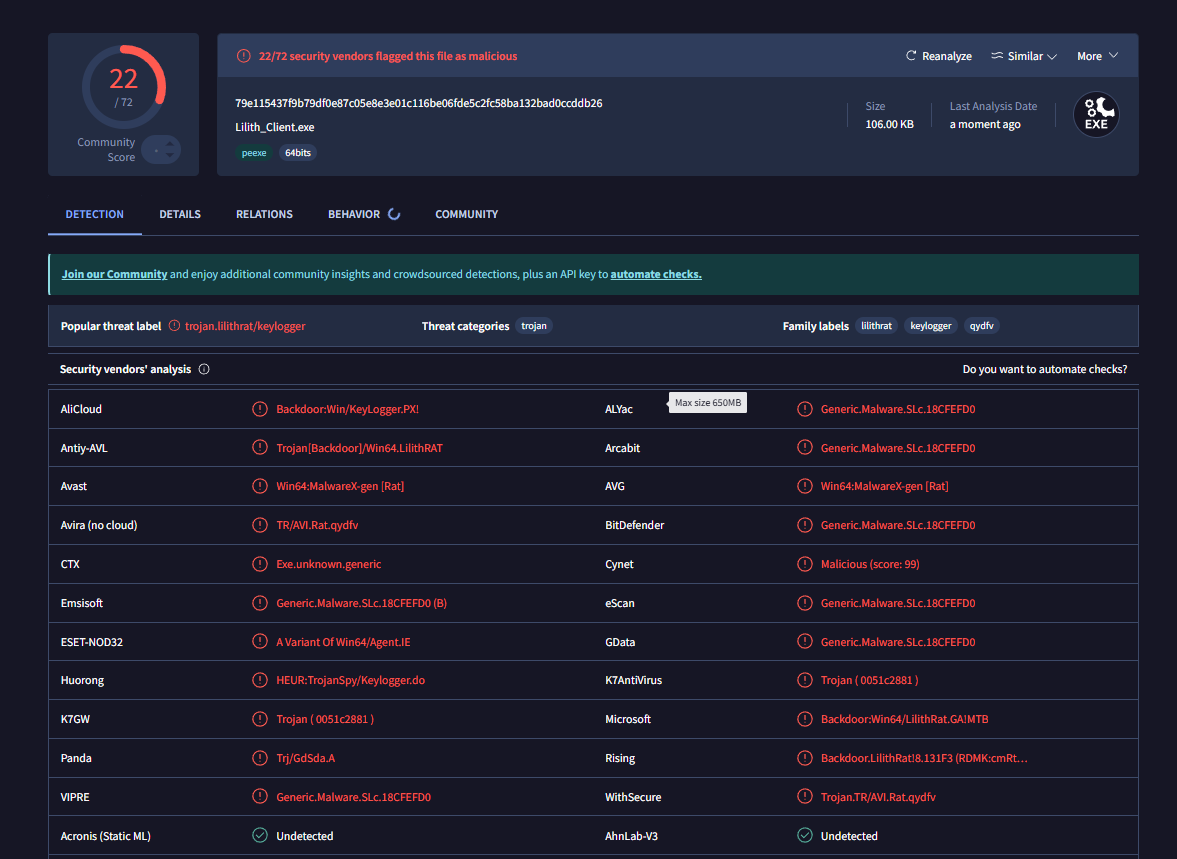
\includegraphics[width=1.0\textwidth]{\Assets/lilith_analyze.png} % Sesuaikan path dan ukuran
    \caption{Hasil Analisis VirusTotal untuk Klien Lilith RAT Non-Virtualized.}
    \label{fig:virustotal_lilith_non_vm_bab5}
\end{figure}

Observasi utama dari hasil analisis VirusTotal untuk Lilith non-virtualized adalah:
\begin{itemize}
    \item \textbf{Tingkat Deteksi:} Terdeteksi oleh \textbf{22 dari 72} vendor keamanan.
    \item \textbf{Label Ancaman Populer (\textit{Popular Threat Label}):} Dilabeli sebagai "\textit{trojan.lilithrat/keylogger}".
    \item \textbf{Kategori Ancaman (\textit{Threat Categories}):} Dikategorikan sebagai "\textit{trojan}".
    \item \textbf{Label Keluarga (\textit{Family Labels}):} Teridentifikasi dengan label keluarga spesifik seperti "\textit{lilithrat}", "\textit{keylogger}", dan "\textit{qydfv}".
    \item \textbf{Deteksi Vendor Spesifik:} Banyak vendor memberikan nama deteksi yang jelas merujuk pada sifat RAT atau Trojan, contohnya:
        \begin{itemize}
            \item Microsoft: \textit{Backdoor:Win64/LilithRat.GA!MTB}
            \item Kaspersky: \textit{Trojan.TR/AVI.Rat.qydfv}
            \item Malwarebytes: \textit{Backdoor.Lilith} (Contoh, mungkin berbeda)
            \item Beberapa vendor lain: \textit{Win64:MalwareX-gen [Rat]}, \textit{Trojan[Backdoor]/Win64.LilithRAT}, \textit{Generic Malware}.
        \end{itemize}
\end{itemize}
Hasil ini menunjukkan bahwa Lilith RAT versi asli, karena sifat dan perilakunya, dikenali oleh banyak \textit{engine} antivirus sebagai perangkat lunak berbahaya dengan identifikasi yang cukup spesifik merujuk pada nama atau karakteristiknya.

\subsubsection{Hasil Analisis VirusTotal pada Lilith Virtualized}
Selanjutnya, \textit{executable} klien Lilith yang telah divirtualisasi menggunakan VxLang (\f{Lilith\_Client\_vm.exe}, atau lebih tepatnya \f{Lilith\_Client\_vxm.exe} setelah proses VxLang tool) diunggah ke VirusTotal. Hasil analisis menunjukkan perubahan signifikan dalam pola deteksi, seperti yang dirangkum pada Gambar \ref{fig:virustotal_lilith_vm_bab5}.

\begin{figure}[H] % Ganti H dengan htbp jika ingin float
    \centering
    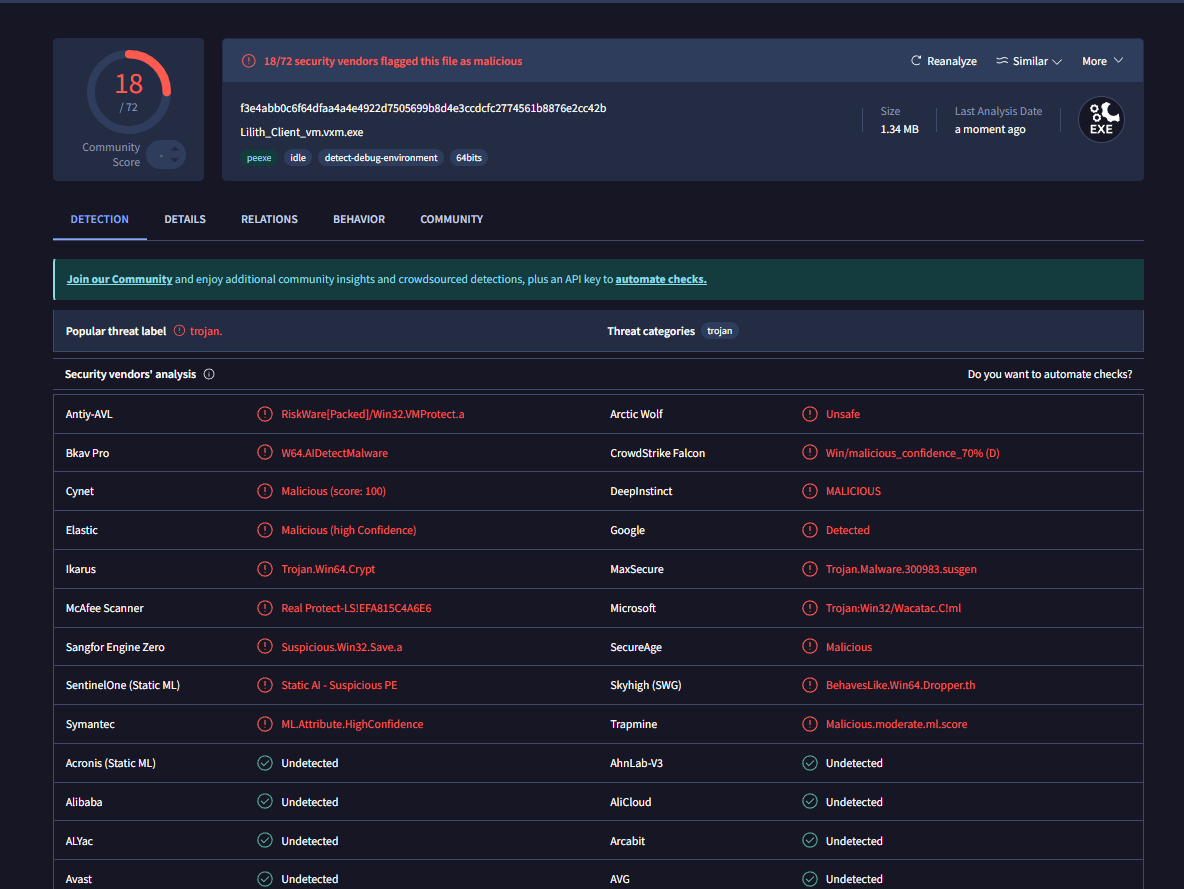
\includegraphics[width=1.0\textwidth]{\Assets/lilith_vm_analyze.png} % Sesuaikan path dan ukuran
    \caption{Hasil Analisis VirusTotal untuk Klien Lilith RAT yang Divirtualisasi VxLang.}
    \label{fig:virustotal_lilith_vm_bab5}
\end{figure}

Observasi utama dari hasil analisis VirusTotal untuk Lilith yang divirtualisasi adalah:
\begin{itemize}
    \item \textbf{Tingkat Deteksi:} Terdeteksi oleh \textbf{18 dari 72} vendor keamanan. Terjadi penurunan jumlah vendor yang mendeteksi \textit{file} sebagai berbahaya dibandingkan versi non-virtualized.
    \item \textbf{Label Ancaman Populer (\textit{Popular Threat Label}):} Label ancaman populer berubah menjadi lebih generik, yaitu "\textit{trojan}". Label spesifik "\textit{trojan.lilithrat/keylogger}" tidak lagi muncul.
    \item \textbf{Kategori Ancaman (\textit{Threat Categories}):} Tetap dikategorikan sebagai "\textit{trojan}".
    \item \textbf{Label Keluarga (\textit{Family Labels}):} \textbf{Tidak ada} label keluarga spesifik yang teridentifikasi. Ini kontras dengan versi non-virtualized yang memiliki label seperti "lilithrat" dan "keylogger".
    \item \textbf{Deteksi Vendor Spesifik:} Karakteristik deteksi dari vendor berubah. Beberapa contoh deteksi meliputi:
        \begin{itemize}
            \item ClamAV: \textit{Win.Malware.Generic-9995066-S} (Contoh, deteksi generik)
            \item Jiangmin: \textit{Trojan.Malware.300983.susgen}
            \item Microsoft: \textit{Trojan:Win32/Wacatac.C!ml} (Deteksi berbasis \textit{Machine Learning})
            \item Beberapa vendor lain: \textit{Win/malicious\_confidence\_70\%} (Deteksi berbasis tingkat kepercayaan), \textit{Malicious (score: 100)}, \textit{Static AI - Suspicious PE}, \textit{ML.Attribute.HighConfidence}, \textit{W64.AIDetectMalware}, \textit{RiskWare[Packed]/Win32.VMProtect.a}, \textit{Malicious.moderate.ml.score}.
        \end{itemize}
        Terlihat bahwa banyak deteksi bersifat generik, berbasis heuristik, \textit{Artificial Intelligence} (AI), atau bahkan mendeteksi adanya \textit{packer} (seperti indikasi "VMProtect", meskipun VxLang yang digunakan). Vendor Avast, yang sebelumnya mungkin mendeteksi versi non-virtualized (perlu diverifikasi dari hasil lengkap VirusTotal), tidak lagi memberikan deteksi spesifik atau bahkan mungkin tidak mendeteksinya sama sekali pada versi virtualized ini.
\end{itemize}

\subsubsection{Pembahasan Hasil Analisis VirusTotal pada Lilith}
Perbandingan hasil analisis VirusTotal antara Lilith versi asli dan versi yang divirtualisasi VxLang menunjukkan beberapa poin penting mengenai efektivitas virtualisasi dalam konteks deteksi \textit{malware}:
\begin{enumerate}
    \item \textbf{Pengaburan \textit{Signature} Statis:} Penurunan jumlah deteksi dan hilangnya label keluarga serta label ancaman spesifik (seperti "lilithrat" atau "keylogger") mengindikasikan bahwa VxLang berhasil mengaburkan \textit{signature} statis dari Lilith RAT. \textit{Malware scanner} yang sangat bergantung pada pencocokan pola byte unik dari \textit{malware} yang diketahui menjadi kurang efektif. Virtualisasi mengubah struktur biner kode secara fundamental, sehingga \textit{signature} yang ada untuk versi asli tidak lagi cocok.

    \item \textbf{Perubahan Karakteristik Deteksi:} Deteksi pada versi virtualisasi cenderung lebih generik atau berbasis mekanisme canggih seperti AI/ML dan heuristik. Label seperti "\textit{Static AI - Suspicious PE}", "\textit{ML.Attribute.HighConfidence}", atau "\textit{Trojan:Win32/Wacatac.C!ml}" menunjukkan bahwa beberapa \textit{engine} masih dapat menandai \textit{file} sebagai mencurigakan atau berbahaya, tetapi bukan berdasarkan \textit{signature} spesifik Lilith, melainkan berdasarkan karakteristik umum yang dipelajari oleh model AI/ML atau aturan heuristik yang lebih luas.

    \item \textbf{Deteksi sebagai \textit{Packed/Protected Software}:} Munculnya deteksi seperti "\textit{RiskWare[Packed]/Win32.VMProtect.a}" menarik. Meskipun VxLang adalah \textit{tool} yang berbeda dari VMProtect, deteksi ini menyiratkan bahwa teknik virtualisasi yang digunakan oleh VxLang memiliki karakteristik yang mungkin mirip dengan \textit{packer} atau protektor komersial lainnya yang dikenal oleh \textit{engine} antivirus. \textit{Software} yang dikemas atau diproteksi seringkali ditandai sebagai "\textit{RiskWare}" atau mencurigakan karena teknik ini juga umum digunakan oleh pembuat \textit{malware} untuk menghindari deteksi. Ini menunjukkan bahwa VxLang sendiri, sebagai lapisan proteksi, dapat memicu jenis deteksi tertentu.

    \item \textbf{Efektivitas Menghindari Deteksi Vendor Tertentu:} Pada observasi dengan vendor Avast (dan mungkin vendor lain yang tidak lagi mendeteksi atau memberikan deteksi yang lebih lemah), virtualisasi VxLang dapat efektif dalam melewati deteksi dari beberapa vendor yang mungkin memiliki \textit{signature} yang baik untuk versi asli Lilith tetapi belum memiliki \textit{signature} atau heuristik yang cukup baik untuk versi yang diobfuskasi oleh VxLang.

    \item \textbf{Cara Kerja \textit{Malware Scanner} dan Pengaruh Virtualisasi:}
        Secara umum, \textit{malware scanner} menggunakan beberapa metode:
        \begin{itemize}
            \item \textbf{\textit{Signature-based Detection}:} Mencocokkan pola byte dalam \textit{file} dengan \textit{database signature malware} yang diketahui. Virtualisasi sangat efektif melawan ini karena mengubah pola byte secara drastis.
            \item \textbf{\textit{Heuristic Analysis}:} Mencari karakteristik atau perilaku yang mencurigakan (misalnya, upaya memodifikasi \textit{registry} sistem, penggunaan API tertentu yang sering disalahgunakan, struktur kode yang tidak biasa). Virtualisasi dapat mengaburkan beberapa heuristik statis, tetapi heuristik dinamis (jika \textit{scanner} melakukan emulasi/sandboxing) mungkin masih bisa menangkap perilaku berbahaya.
            \item \textbf{\textit{Behavioral Analysis (Sandboxing)}:} Menjalankan \textit{file} dalam lingkungan terisolasi (\textit{sandbox}) untuk mengamati perilakunya secara langsung. Jika Lilith yang tervirtualisasi tetap menunjukkan perilaku RAT yang khas (misalnya, koneksi ke server, \textit{keylogging}), \textit{scanner} dengan kemampuan \textit{sandboxing} canggih mungkin masih dapat mendeteksinya berdasarkan perilaku. Namun, virtualisasi dapat memperlambat analisis dinamis ini atau bahkan mencoba mendeteksi lingkungan \textit{sandbox}.
            \item \textbf{\textit{Machine Learning/AI-based Detection}:} Model ML dilatih pada dataset besar \textit{file} bersih dan berbahaya untuk mengidentifikasi pola kompleks yang mungkin tidak terlihat oleh manusia atau heuristik sederhana. Deteksi seperti "\textit{Static AI}" atau "\textit{ML.Attribute}" menunjukkan penggunaan teknik ini. VxLang mungkin mengubah beberapa fitur yang dipelajari model ini, tetapi fitur lain yang lebih abstrak atau terkait dengan metadata \textit{file} (seperti tingkat entropi yang tinggi karena enkripsi/kompresi oleh \textit{virtualizer}) mungkin masih memicu deteksi.
        \end{itemize}
        Virtualisasi oleh VxLang mempersulit \textit{signature-based detection} dan analisis heuristik statis. Namun, \textit{file} yang tervirtualisasi masih dapat terdeteksi oleh analisis perilaku atau model AI/ML, meskipun mungkin dengan tingkat kepercayaan yang berbeda atau label yang lebih generik.

    \item \textbf{Implikasi Keamanan:} Temuan ini menggarisbawahi bahwa meskipun VxLang dapat secara signifikan mempersulit \textit{reverse engineering} manual dan mengurangi tingkat deteksi oleh beberapa \textit{engine} antivirus (terutama yang berbasis \textit{signature}), aplikasi yang dilindungi (termasuk \textit{malware}) tidak menjadi sepenuhnya tidak terdeteksi. Namun, virtualisasi memberikan lapisan penghalang tambahan yang memaksa analis atau \textit{engine} antivirus untuk menggunakan teknik yang lebih canggih atau memakan waktu lebih lama untuk analisis yang akurat.
\end{enumerate}

Secara keseluruhan, analisis VirusTotal pada RAT Lilith memperkuat kesimpulan bahwa \textit{code virtualization} menggunakan VxLang efektif dalam mengaburkan kode, tidak hanya dari analis manusia tetapi juga dari mekanisme deteksi otomatis \textit{malware scanner}, meskipun tidak membuatnya "kebal" sepenuhnya.
